% !TEX root = ../presentation.tex
% !BIB program = biber
% !TEX program = xelatex

\section{a brief overview of unsupervised speech representation learning}

\begin{frame}
    \frametitle{Development of SSL for speech}
    \begingroup
    \small% \small in 11pt base font is 10pt
    \begin{columns}[t]
        \hspace{0.025\textwidth}
        \begin{column}{0.20\textwidth}
            \begin{figure}[\textwidth]
                \centering
                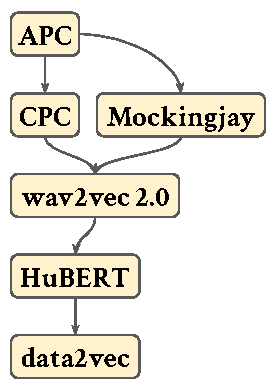
\includegraphics[width=\textwidth]{figures/brief-flow-0.pdf}
            \end{figure}
        \end{column}
        {\textcolor{black!40}{\vrule{}}}
        % \begin{column}{0.4\txtwidth}
            % \vspace{0.1\textheight}
            % {\footnotesize #3}
        % \end{column}
        % \hfill
        \hspace{0.050\textwidth}
        \begin{column}{0.65\textwidth}
            \begin{figure}[\textwidth]
                \centering
                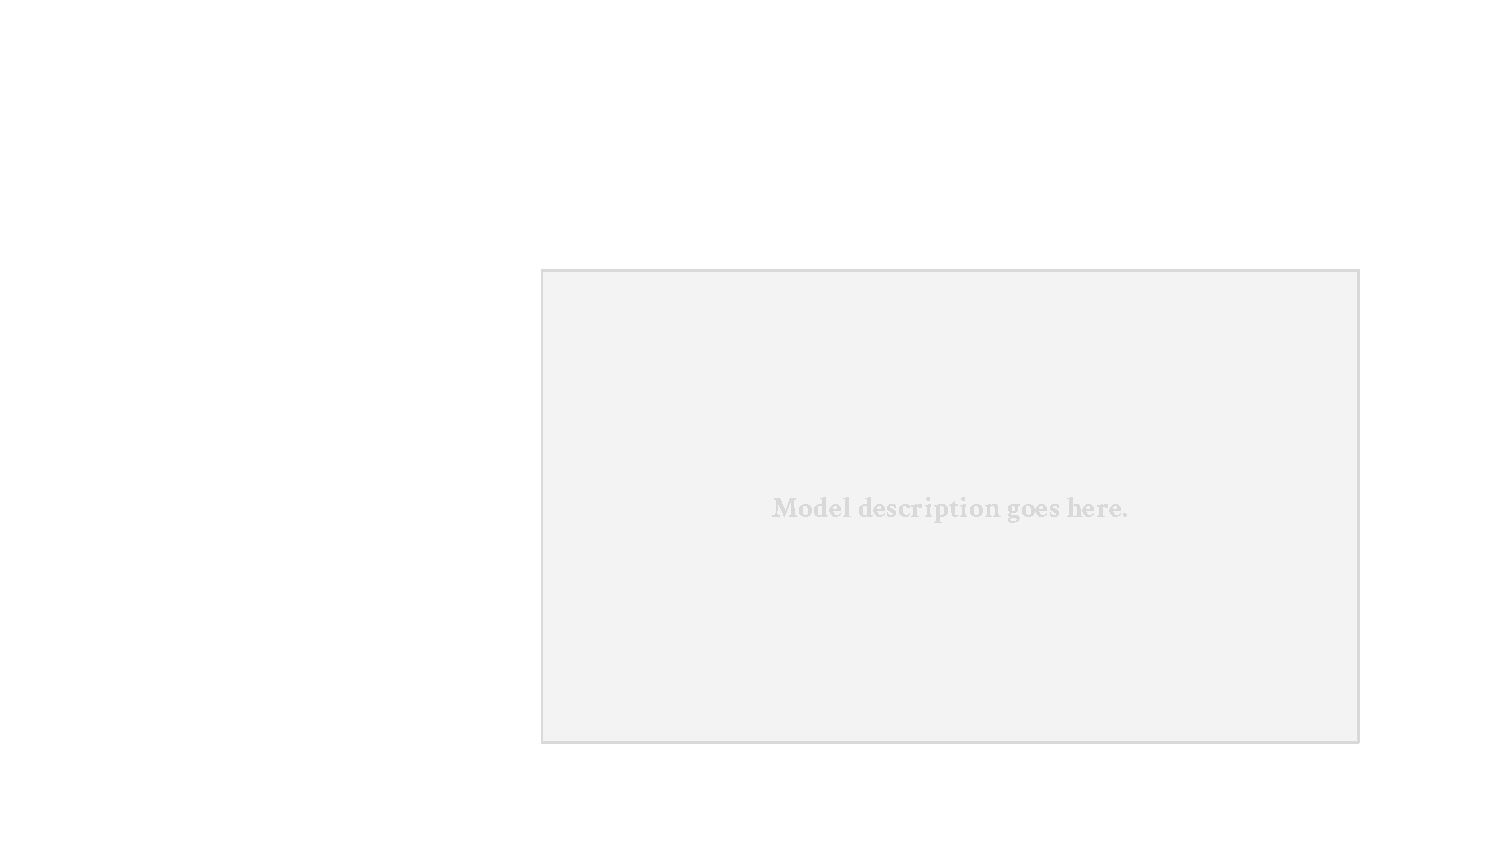
\includegraphics[width=\textwidth]{figures/brief-model-0.pdf}
            \end{figure}
        \end{column}
        % \hfill
        \hspace{0.020\textwidth}
    \end{columns}
    \endgroup
\end{frame}


\newcommand{\presentationbriefslide}[3]{%
    \begin{frame}
        \frametitle{#2}
        \begin{columns}[t]
            \hspace{0.025\textwidth}
            \begin{column}{0.20\textwidth}
                \begin{figure}[\textwidth]
                    \centering
                    \includegraphics[width=\textwidth]{figures/brief-flow-#1.pdf}
                \end{figure}
            \end{column}
            {\textcolor{black!40}{\vrule{}}}
            \begin{column}{0.4\textwidth}
                {\vspace{0.1\textheight}#3}
            \end{column}
            \begin{column}{0.30\textwidth}
                \begin{figure}[\textwidth]
                    \centering
                    \includegraphics[width=\textwidth]{figures/brief-model-#1.pdf}
                \end{figure}
            \end{column}
            \hspace{0.020\textwidth}
        \end{columns}
    \end{frame}
}

\presentationbriefslide{0}{Development of self-supervised learning for speech}{%
    % \begin{itemize}
        % \item {\bfseries \color{black} 2019}: APC \cite{}.
        % \item {\bfseries \color{black} 2020}: CPC \cite{}.
        % \item {\bfseries \color{black} 2020}: Mockingjay \cite{}.
        % \item {\bfseries \color{black} 2019}: Wav2vec \cite{schneider_wav2vec_2019}.
        % \item {\bfseries \color{black} 2021}: HuBERT \cite{hsu_hubert_2021}.
        % \item {\bfseries \color{black} 2022}: data2vec \cite{baevski_data2vec_2022}
    % \end{itemize}
}

\presentationbriefslide{1}{Autoregressive Predictive Coding (APC)}{%
    \begin{itemize}
        \item {\bfseries \color{black} Task}: Predict future inputs.
        \item {\bfseries \color{black} Input/target}: Log-mel spectrogram.
        \item {\bfseries \color{black} Architecture}: RNN/Transformer decoder.
        \item {\bfseries \color{black} Slow features}: Predict $k$ steps ahead.
    \end{itemize}
}

\presentationbriefslide{2}{Autoregressive Predictive Coding (APC)}{%
    \begin{itemize}
        \item {\bfseries \color{black} Challenges}:
        \begin{itemize}
            \item Encodes only past inputs.
            \item Uses the input as target.
        \end{itemize}
    \end{itemize}
}

\presentationbriefslide{3}{Mockingjay}{%
    \begin{itemize}
        \item {\bfseries \color{black} Task}: Reconstruct masked inputs.
        \item {\bfseries \color{black} Architecture}: Transformer encoder.
        \item {\bfseries \color{black} Masking}: 
        \begin{itemize}
            \item $X$\% at random. (Mockingjay)
            \item $X$\% + $N$ consecutive (wav2vec 2.0)
            \item SpecAugment (Masked RNN)
        \end{itemize}
    \end{itemize}
}

\presentationbriefslide{4}{Mockingjay}{%

}

\presentationbriefslide{5}{Mockingjay}{%

}

\presentationbriefslide{6}{Mockingjay}{%

}

\presentationbriefslide{7}{Mockingjay}{%

}

\presentationbriefslide{8}{Mockingjay}{%

}

\presentationbriefslide{9}{Mockingjay}{%

}

\presentationbriefslide{10}{Mockingjay}{%

}

\presentationbriefslide{11}{Mockingjay}{%

}

\presentationbriefslide{12}{Mockingjay}{%

}

\presentationbriefslide{13}{Mockingjay}{%

}

\presentationbriefslide{14}{Mockingjay}{%

}

\presentationbriefslide{15}{Mockingjay}{%

}

\presentationbriefslide{16}{Mockingjay}{%

}


% TODO: Add slides with overview of latent variable models.


